
\documentclass[border=10pt, 12pt]{standalone}
\usepackage[svgnames]{xcolor}
\usepackage{amsmath}
\usepackage{pgfplots}
\pgfplotsset{compat=newest}
\usepackage[sfdefault]{FiraSans}
\usepackage{FiraMono}
\renewcommand*\familydefault{\sfdefault}
\begin{document}
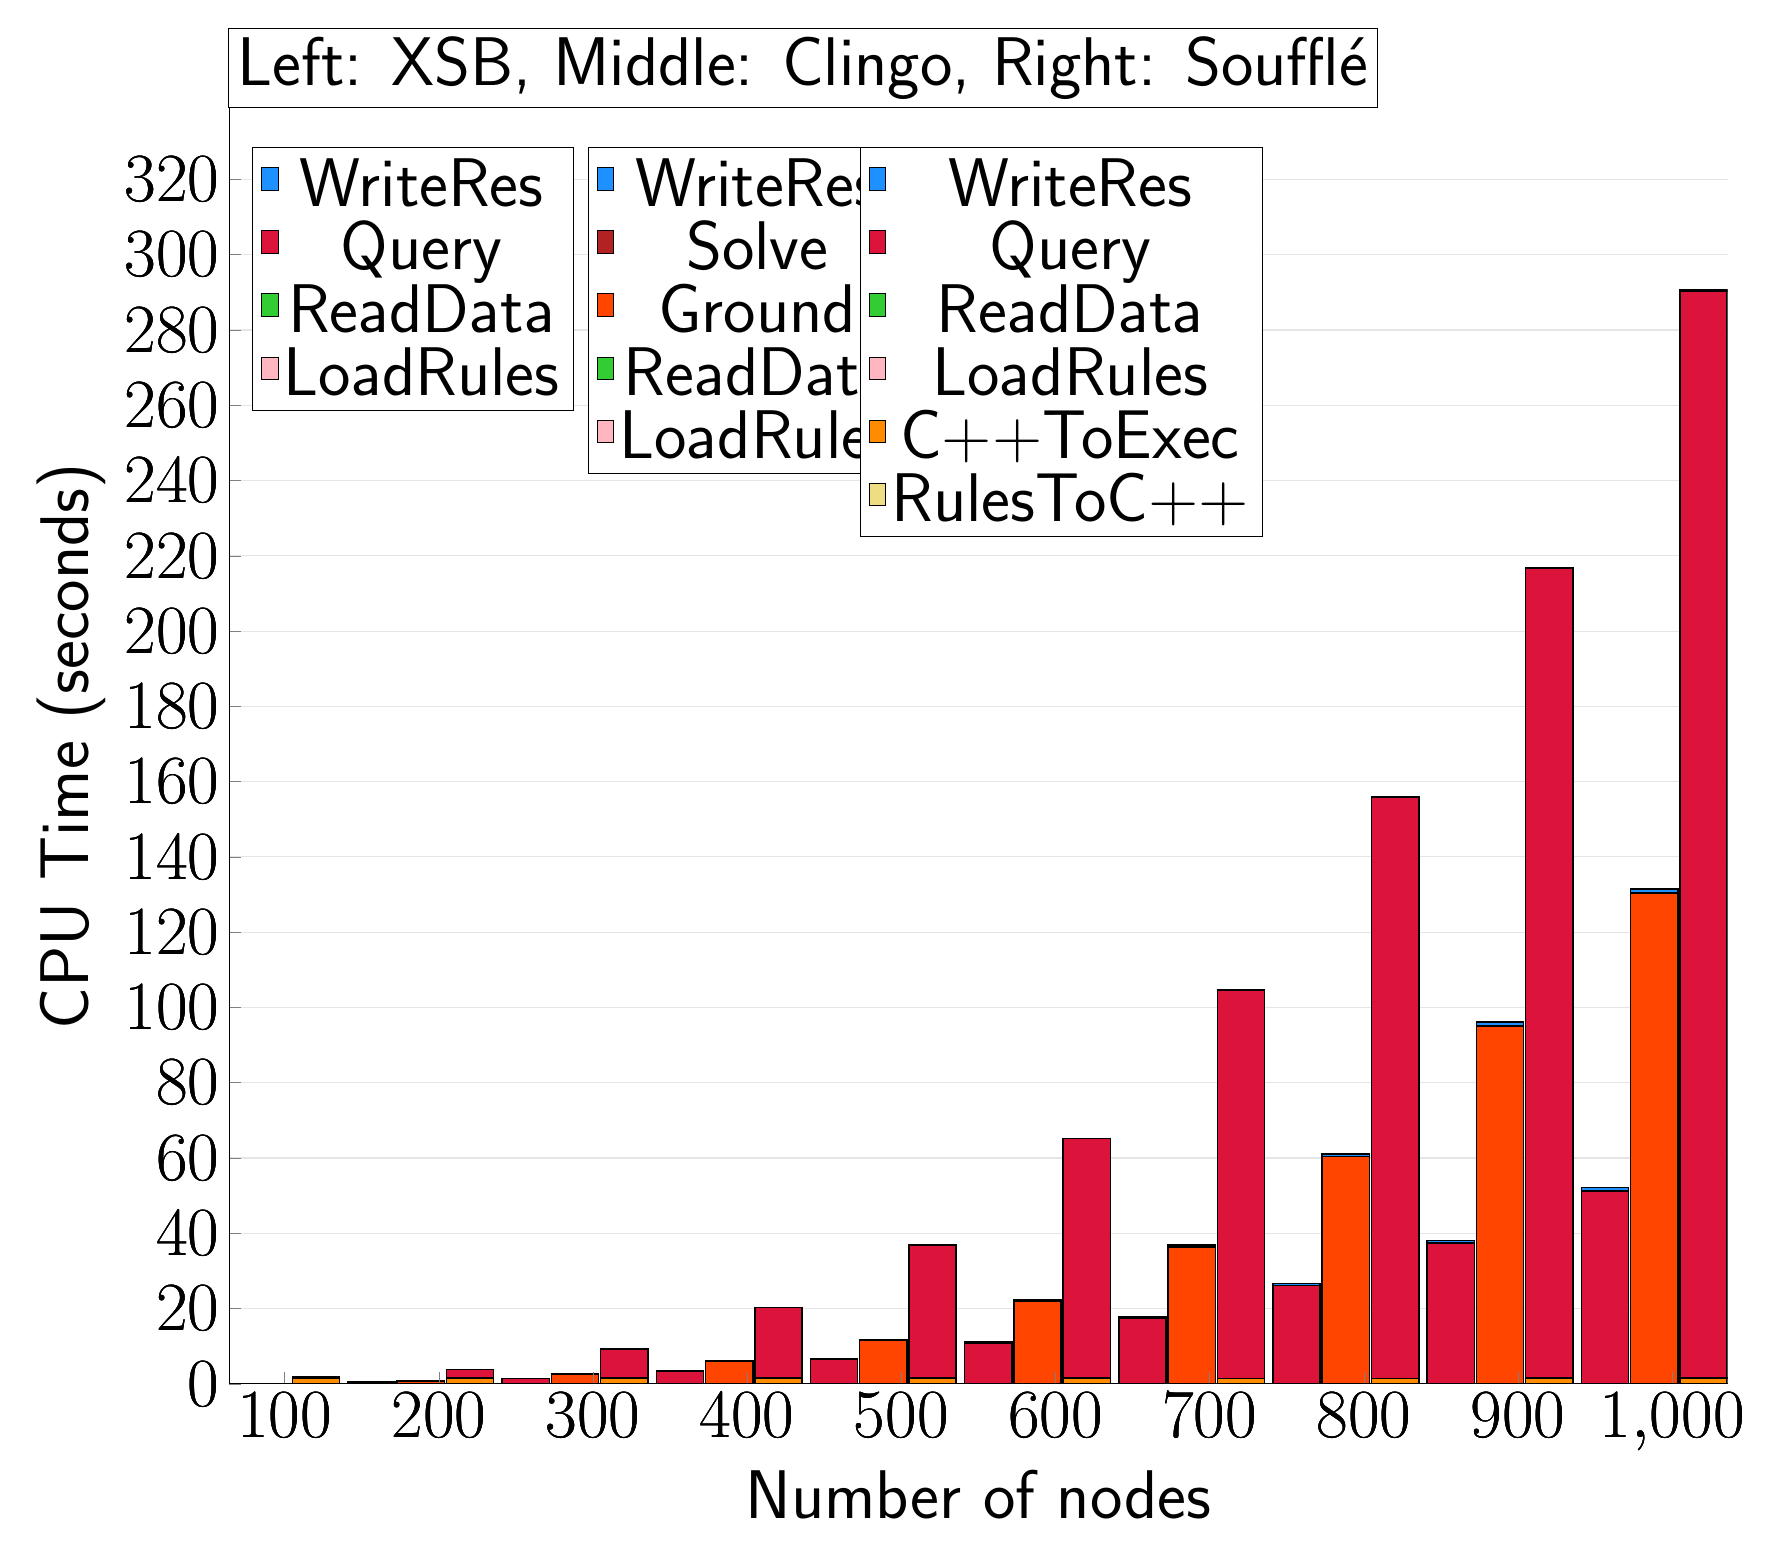
\begin{tikzpicture}
                        \begin{axis}[bar shift=-24.3pt, 
   ybar stacked,
   width=1.7\textwidth,
   bar width=0.6cm,
   ymajorgrids, tick align=inside,
   major grid style={draw=gray!20},
   xtick=data,
   ymin=0, ymax=338.8692,
   axis x line*=bottom,
   axis y line*=left,
   enlarge x limits=0.04,
   legend style={
       at={(0.23, 0.97)},
       anchor=north east,
       legend columns=1,
       font=\Huge,
   },
   ylabel={CPU Time (seconds)},
   xlabel={Number of nodes},
   label style={font=\Huge},
   tick label style={font=\Huge},
]
\addlegendimage{fill=DodgerBlue, draw=black, line width=0.2pt}
\addlegendentry{WriteRes}
\addlegendimage{fill=Crimson, draw=black, line width=0.2pt}
\addlegendentry{Query}
\addlegendimage{fill=LimeGreen, draw=black, line width=0.2pt}
\addlegendentry{ReadData}
\addlegendimage{fill=LightPink, draw=black, line width=0.2pt}
\addlegendentry{LoadRules}
\addplot +[fill=LightPink, draw=black, line width=0.55pt] coordinates {
(100, 0.0005554000000000002)
(200, 0.0005518000000000002)
(300, 0.0005580000000000002)
(400, 0.0005523999999999998)
(500, 0.0005491999999999998)
(600, 0.000553)
(700, 0.0005515999999999999)
(800, 0.0005547999999999996)
(900, 0.0005565999999999997)
(1000, 0.0005629999999999999)
};
\addplot +[fill=LimeGreen, draw=black, line width=0.55pt] coordinates {
(100, 0.0001990000000000004)
(200, 0.00027600000000000015)
(300, 0.0003568000000000002)
(400, 0.00044320000000000004)
(500, 0.0005138000000000003)
(600, 0.0005938)
(700, 0.0006752000000000001)
(800, 0.0007479999999999998)
(900, 0.0008426)
(1000, 0.0009039999999999992)
};
\addplot +[fill=Crimson, draw=black, line width=0.55pt] coordinates {
(100, 0.0529404)
(200, 0.4258976)
(300, 1.3886992)
(400, 3.3225496)
(500, 6.491732600000001)
(600, 10.8728596)
(700, 17.325140600000005)
(800, 26.163236599999998)
(900, 37.374866000000004)
(1000, 51.22737500000001)
};
\addplot +[fill=DodgerBlue, draw=black, line width=0.55pt] coordinates {
(100, 0.010683600000000001)
(200, 0.032202600000000026)
(300, 0.06599320000000009)
(400, 0.13044899999999987)
(500, 0.18336400000000008)
(600, 0.3010274000000003)
(700, 0.4191758)
(800, 0.4942852000000002)
(900, 0.6579791999999998)
(1000, 0.9104848000000019)
};
\end{axis}

\begin{axis}[bar shift=-6.5pt, 
   ybar stacked,
   width=1.7\textwidth,
   bar width=0.6cm,
   ymajorgrids, tick align=inside,
   major grid style={draw=none},
   xtick=data,
   ymin=0, ymax=338.8692,
   axis x line*=none,
   axis y line*=none,
   enlarge x limits=0.04,
   legend style={
       at={(0.454, 0.97)},
       anchor=north east,
       legend columns=1,
       font=\Huge,
   },
   label style={font=\Huge},
   tick label style={font=\Huge},
]
\addlegendimage{fill=DodgerBlue, draw=black, line width=0.2pt}
\addlegendentry{WriteRes}
\addlegendimage{fill=FireBrick, draw=black, line width=0.2pt}
\addlegendentry{Solve}
\addlegendimage{fill=OrangeRed, draw=black, line width=0.2pt}
\addlegendentry{Ground}
\addlegendimage{fill=LimeGreen, draw=black, line width=0.2pt}
\addlegendentry{ReadData}
\addlegendimage{fill=LightPink, draw=black, line width=0.2pt}
\addlegendentry{LoadRules}
\addplot +[fill=LightPink, draw=black, line width=0.55pt] coordinates {
(100, 0.0)
(200, 0.0)
(300, 0.0)
(400, 0.0)
(500, 0.0)
(600, 0.0)
(700, 0.0)
(800, 0.0)
(900, 0.0)
(1000, 0.0)
};
\addplot +[fill=LimeGreen, draw=black, line width=0.55pt] coordinates {
(100, 0.0)
(200, 0.0)
(300, 0.0)
(400, 0.0)
(500, 0.0)
(600, 0.0)
(700, 0.0)
(800, 0.0)
(900, 0.0)
(1000, 0.0)
};
\addplot +[fill=OrangeRed, draw=black, line width=0.55pt] coordinates {
(100, 0.09400000000000003)
(200, 0.73)
(300, 2.5780000000000003)
(400, 6.012)
(500, 11.458)
(600, 21.952)
(700, 36.332)
(800, 60.346000000000004)
(900, 95.1)
(1000, 130.30599999999998)
};
\addplot +[fill=FireBrick, draw=black, line width=0.55pt] coordinates {
(100, 0.0)
(200, 0.0040000000000000036)
(300, 0.005999999999999872)
(400, 0.00799999999999983)
(500, 0.01599999999999966)
(600, 0.019999999999999574)
(700, 0.03200000000000114)
(800, 0.03599999999999852)
(900, 0.049999999999998976)
(1000, 0.06000000000000022)
};
\addplot +[fill=DodgerBlue, draw=black, line width=0.55pt] coordinates {
(100, 0.01599999999999996)
(200, 0.04200000000000004)
(300, 0.10800000000000023)
(400, 0.18400000000000052)
(500, 0.2840000000000005)
(600, 0.41400000000000226)
(700, 0.5579999999999996)
(800, 0.7220000000000033)
(900, 0.9280000000000019)
(1000, 1.1399999999999975)
};
\end{axis}

\begin{axis}[bar shift=11.3pt, 
   ybar stacked,
   width=1.7\textwidth,
   bar width=0.6cm,
   ymajorgrids, tick align=inside,
   major grid style={draw=none},
   xtick=data,
   ymin=0, ymax=338.8692,
   axis x line*=none,
   axis y line*=none,
   enlarge x limits=0.04,
   legend style={
       at={(0.69, 0.97)},
       anchor=north east,
       legend columns=1,
       font=\Huge,
   },
   label style={font=\Huge},
   tick label style={font=\Huge},
]
\addlegendimage{fill=DodgerBlue, draw=black, line width=0.2pt}
\addlegendentry{WriteRes}
\addlegendimage{fill=Crimson, draw=black, line width=0.2pt}
\addlegendentry{Query}
\addlegendimage{fill=LimeGreen, draw=black, line width=0.2pt}
\addlegendentry{ReadData}
\addlegendimage{fill=LightPink, draw=black, line width=0.2pt}
\addlegendentry{LoadRules}
\addlegendimage{fill=DarkOrange, draw=black, line width=0.2pt}
\addlegendentry{C++ToExec}
\addlegendimage{fill=LightGoldenrod, draw=black, line width=0.2pt}
\addlegendentry{RulesToC++}
\addplot +[fill=LightGoldenrod, draw=black, line width=0.55pt] coordinates {
(100, 0.0020000000000000005)
(200, 0.0020000000000000005)
(300, 0.007999999999999997)
(400, 0.0020000000000000005)
(500, 0.0020000000000000005)
(600, 0.0020000000000000005)
(700, 0.0)
(800, 0.004000000000000001)
(900, 0.0)
(1000, 0.0)
};
\addplot +[fill=DarkOrange, draw=black, line width=0.55pt] coordinates {
(100, 1.482)
(200, 1.482)
(300, 1.48)
(400, 1.48)
(500, 1.482)
(600, 1.486)
(700, 1.472)
(800, 1.47)
(900, 1.4780000000000002)
(1000, 1.502)
};
\addplot +[fill=LightPink, draw=black, line width=0.55pt] coordinates {
(100, 0.0001818)
(200, 0.00017740000000000003)
(300, 0.00018700000000000002)
(400, 0.00018899999999999999)
(500, 0.00020800000000000001)
(600, 0.00020740000000000003)
(700, 0.0001186)
(800, 0.0001024)
(900, 0.00023579999999999999)
(1000, 0.00018680000000000001)
};
\addplot +[fill=LimeGreen, draw=black, line width=0.55pt] coordinates {
(100, 0.000792)
(200, 0.0011237999999999999)
(300, 0.0014081999999999999)
(400, 0.0020178)
(500, 0.0024934)
(600, 0.003045)
(700, 0.0023056)
(800, 0.0019614)
(900, 0.0046672)
(1000, 0.0032714)
};
\addplot +[fill=Crimson, draw=black, line width=0.55pt] coordinates {
(100, 0.3054582)
(200, 2.297596)
(300, 7.766288)
(400, 18.82078)
(500, 35.3274)
(600, 63.66976)
(700, 103.03400000000002)
(800, 154.2942)
(900, 215.1904)
(1000, 288.8692)
};
\addplot +[fill=DodgerBlue, draw=black, line width=0.55pt] coordinates {
(100, 0.002468)
(200, 0.0089116)
(300, 0.0195672)
(400, 0.034351200000000005)
(500, 0.0533714)
(600, 0.07718799999999999)
(700, 0.1043056)
(800, 0.1356366)
(900, 0.17171799999999998)
(1000, 0.2105976)
};
\end{axis}


\node[anchor=south, draw, fill=white] at (rel axis cs:0.42,1) {\Huge Left: XSB, Middle: Clingo, Right: Soufflé};
\end{tikzpicture}
\end{document}
                    